% 若编译失败,且生成 .synctex(busy) 辅助文件,可能有两个原因:
% 1. 需要插入的图片不存在:Ctrl + F 搜索 'figure' 将这些代码注释/删除掉即可
% 2. 路径/文件名含中文或空格:更改路径/文件名即可

% --------------------- 文章宏包及相关设置 --------------------- %
% >> ------------------ 文章宏包及相关设置 ------------------ << %
% 设定文章类型与编码格式
\documentclass[UTF8]{article}		

% 物理实验报告所需的其它宏包
\usepackage{ulem}   % \uline 下划线支持

% 本 .tex 专属的宏定义
    \def\V{\ \mathrm{V}}
    \def\mV{\ \mathrm{mV}}
    \def\kV{\ \mathrm{KV}}
    \def\KV{\ \mathrm{KV}}
    \def\MV{\ \mathrm{MV}}
    \def\A{\ \mathrm{A}}
    \def\mA{\ \mathrm{mA}}
    \def\kA{\ \mathrm{KA}}
    \def\KA{\ \mathrm{KA}}
    \def\MA{\ \mathrm{MA}}
    \def\O{\ \Omega}
    \def\mO{\ \Omega}
    \def\kO{\ \mathrm{K}\Omega}
    \def\KO{\ \mathrm{K}\Omega}
    \def\MO{\ \mathrm{M}\Omega}
    \def\Hz{\ \mathrm{Hz}}

% 自定义宏定义
    \def\N{\mathbb{N}}
    \def\F{\mathbb{F}}
    \def\Z{\mathbb{Z}}
    \def\Q{\mathbb{Q}}
    \def\R{\mathbb{R}}
    \def\C{\mathbb{C}}
    \def\T{\mathbb{T}}
    \def\S{\mathbb{S}}
    %\def\A{\mathbb{A}}
    \def\I{\mathscr{I}}
    \def\d{\mathrm{d}}
    \def\p{\partial}


% 导入基本宏包
    \usepackage[UTF8]{ctex}     % 设置文档为中文语言
    \usepackage{hyperref}  % 宏包:自动生成超链接 (此宏包与标题中的数学环境冲突)
    \hypersetup{
        colorlinks=true,    % false:边框链接 ; true:彩色链接
        citecolor={blue},    % 文献引用颜色
        linkcolor={blue},   % 目录 (我们在目录处单独设置),公式,图表,脚注等内部链接颜色
        urlcolor={magenta},    % 网页 URL 链接颜色,包括 \href 中的 text
        % cyan 浅蓝色 
        % magenta 洋红色
        % yellow 黄色
        % black 黑色
        % white 白色
        % red 红色
        % green 绿色
        % blue 蓝色
        % gray 灰色
        % darkgray 深灰色
        % lightgray 浅灰色
        % brown 棕色
        % lime 石灰色
        % olive 橄榄色
        % orange 橙色
        % pink 粉红色
        % purple 紫色
        % teal 蓝绿色
        % violet 紫罗兰色
    }
    % \usepackage{docmute}    % 宏包:子文件导入时自动去除导言区,用于主/子文件的写作方式,\include{./51单片机笔记}即可。注:启用此宏包会导致.tex文件capacity受限。
    \usepackage{amsmath}    % 宏包:数学公式
    \usepackage{mathrsfs}   % 宏包:提供更多数学符号
    \usepackage{amssymb}    % 宏包:提供更多数学符号
    \usepackage{pifont}     % 宏包:提供了特殊符号和字体
    \usepackage{extarrows}  % 宏包:更多箭头符号 
    \usepackage{multicol}   % 宏包:支持多栏 

% 文章页面margin设置
    \usepackage[a4paper]{geometry}
        \geometry{top=0.75in}
        \geometry{bottom=0.75in}
        \geometry{left=0.75in}
        \geometry{right=0.75in}   % 设置上下左右页边距
        \geometry{marginparwidth=1.75cm}    % 设置边注距离(注释、标记等)

% 配置数学环境
    \usepackage{amsthm} % 宏包:数学环境配置
    % theorem-line 环境自定义
        \newtheoremstyle{MyLineTheoremStyle}% <name>
            {11pt}% <space above>
            {11pt}% <space below>
            {\kaishu}% <body font> 默认使用正文字体, \kaishu 为楷体
            {}% <indent amount>
            {\bfseries}% <theorem head font> 设置标题项为加粗
            {:\ \ }% <punctuation after theorem head>
            {.5em}% <space after theorem head>
            {\textbf{#1}\thmnumber{#2}\ \ (\,\textbf{#3}\,)}% 设置标题内容顺序
        \theoremstyle{MyLineTheoremStyle} % 应用自定义的定理样式
        \newtheorem{LineTheorem}{Theorem.\,}
    % theorem-block 环境自定义
        \newtheoremstyle{MyBlockTheoremStyle}% <name>
            {11pt}% <space above>
            {11pt}% <space below>
            {\kaishu}% <body font> 使用默认正文字体
            {}% <indent amount>
            {\bfseries}% <theorem head font> 设置标题项为加粗
            {:\\ \indent}% <punctuation after theorem head>
            {.5em}% <space after theorem head>
            {\textbf{#1}\thmnumber{#2}\ \ (\,\textbf{#3}\,)}% 设置标题内容顺序
        \theoremstyle{MyBlockTheoremStyle} % 应用自定义的定理样式
        \newtheorem{BlockTheorem}[LineTheorem]{Theorem.\,} % 使用 LineTheorem 的计数器
    % definition 环境自定义
        \newtheoremstyle{MySubsubsectionStyle}% <name>
            {11pt}% <space above>
            {11pt}% <space below>
            {}% <body font> 使用默认正文字体
            {}% <indent amount>
            {\bfseries}% <theorem head font> 设置标题项为加粗
            {:\\ \indent}% <punctuation after theorem head>
            {0pt}% <space after theorem head>
            {\textbf{#3}}% 设置标题内容顺序
        \theoremstyle{MySubsubsectionStyle} % 应用自定义的定理样式
        \newtheorem{definition}{}

%宏包:有色文本框(proof环境)及其设置
    \usepackage[dvipsnames,svgnames]{xcolor}    %设置插入的文本框颜色
    \usepackage[strict]{changepage}     % 提供一个 adjustwidth 环境
    \usepackage{framed}     % 实现方框效果
        \definecolor{graybox_color}{rgb}{0.95,0.95,0.96} % 文本框颜色。修改此行中的 rgb 数值即可改变方框纹颜色,具体颜色的rgb数值可以在网站https://colordrop.io/ 中获得。(截止目前的尝试还没有成功过,感觉单位不一样)(找到喜欢的颜色,点击下方的小眼睛,找到rgb值,复制修改即可)
        \newenvironment{graybox}{%
        \def\FrameCommand{%
        \hspace{1pt}%
        {\color{gray}\small \vrule width 2pt}%
        {\color{graybox_color}\vrule width 4pt}%
        \colorbox{graybox_color}%
        }%
        \MakeFramed{\advance\hsize-\width\FrameRestore}%
        \noindent\hspace{-4.55pt}% disable indenting first paragraph
        \begin{adjustwidth}{}{7pt}%
        \vspace{2pt}\vspace{2pt}%
        }
        {%
        \vspace{2pt}\end{adjustwidth}\endMakeFramed%
        }

% 外源代码插入设置
    % matlab 代码插入设置
    \usepackage{matlab-prettifier}
        \lstset{style=Matlab-editor}    % 继承 matlab 代码高亮 , 此行不能删去
    \usepackage[most]{tcolorbox} % 引入tcolorbox包 
    \usepackage{listings} % 引入listings包
        \tcbuselibrary{listings, skins, breakable}
        \newfontfamily\codefont{Consolas} % 定义需要的 codefont 字体
        \lstdefinestyle{MatlabStyle_inc}{   % 插入代码的样式
            language=Matlab,
            basicstyle=\small\ttfamily\codefont,    % ttfamily 确保等宽 
            breakatwhitespace=false,
            breaklines=true,
            captionpos=b,
            keepspaces=true,
            numbers=left,
            numbersep=15pt,
            showspaces=false,
            showstringspaces=false,
            showtabs=false,
            tabsize=2,
            xleftmargin=15pt,   % 左边距
            %frame=single, % single 为包围式单线框
            frame=shadowbox,    % shadowbox 为带阴影包围式单线框效果
            %escapeinside=``,   % 允许在代码块中使用 LaTeX 命令 (此行无用)
            %frameround=tttt,    % tttt 表示四个角都是圆角
            framextopmargin=0pt,    % 边框上边距
            framexbottommargin=0pt, % 边框下边距
            framexleftmargin=5pt,   % 边框左边距
            framexrightmargin=5pt,  % 边框右边距
            rulesepcolor=\color{red!20!green!20!blue!20}, % 阴影框颜色设置
            %backgroundcolor=\color{blue!10}, % 背景颜色
        }
        \lstdefinestyle{MatlabStyle_src}{   % 插入代码的样式
            language=Matlab,
            basicstyle=\small\ttfamily\codefont,    % ttfamily 确保等宽 
            breakatwhitespace=false,
            breaklines=true,
            captionpos=b,
            keepspaces=true,
            numbers=left,
            numbersep=15pt,
            showspaces=false,
            showstringspaces=false,
            showtabs=false,
            tabsize=2,
        }
        \newtcblisting{matlablisting}{
            %arc=2pt,        % 圆角半径
            % 调整代码在 listing 中的位置以和引入文件时的格式相同
            top=0pt,
            bottom=0pt,
            left=-5pt,
            right=-5pt,
            listing only,   % 此句不能删去
            listing style=MatlabStyle_src,
            breakable,
            colback=white,   % 选一个合适的颜色
            colframe=black!0,   % 感叹号后跟不透明度 (为 0 时完全透明)
        }
        \lstset{
            style=MatlabStyle_inc,
        }

% table 支持
    \usepackage{booktabs}   % 宏包:三线表
    \usepackage{tabularray} % 宏包:表格排版
    \usepackage{longtable}  % 宏包:长表格

% figure 设置
    \usepackage{graphicx}  % 支持 jpg, png, eps, pdf 图片 
    \usepackage{svg}       % 支持 svg 图片
        \svgsetup{
            % 指向 inkscape.exe 的路径
            inkscapeexe = C:/aa_MySame/inkscape/bin/inkscape.exe, 
            % 一定程度上修复导入后图片文字溢出几何图形的问题
            inkscapelatex = false                 
        }
    \usepackage{subcaption} % 用于子图和小图注  

% 图表进阶设置
    \usepackage{caption}    % 图注、表注
        \captionsetup[figure]{name=图}  
        \captionsetup[table]{name=表}
        \captionsetup{
            labelfont=bf, % 设置标签为粗体
            textfont=bf,  % 设置文本为粗体
            font=small  
        }
    \usepackage{float}     % 图表位置浮动设置 
    \usepackage{etoolbox} % 用于保证图注表注的数学字符为粗体
        \AtBeginEnvironment{figure}{\boldmath} % 图注中的数学字符为粗体
        \AtBeginEnvironment{table}{\boldmath}  % 表注中的数学字符为粗体
        \AtBeginEnvironment{tabular}{\unboldmath}   % 保证表格中的数学字符不受额外影响
% 圆圈序号自定义
    \newcommand*\circled[1]{\tikz[baseline=(char.base)]{\node[shape=circle,draw,inner sep=0.8pt, line width = 0.03em] (char) {\small \bfseries #1};}}   % TikZ solution

% 列表设置
    \usepackage{enumitem}   % 宏包:列表环境设置
        \setlist[enumerate]{
            label=(\arabic*) ,   % 设置序号样式为加粗的 (1) (2) (3)
            ref=\arabic*, % 如果需要引用列表项,这将决定引用格式(这里仍然使用数字)
            itemsep=0pt, parsep=0pt, topsep=0pt, partopsep=0pt, leftmargin=3.5em} 
        \setlist[itemize]{itemsep=0pt, parsep=0pt, topsep=0pt, partopsep=0pt, leftmargin=3.5em}
        \newlist{circledenum}{enumerate}{1} % 创建一个新的枚举环境  
        \setlist[circledenum,1]{  
            label=\protect\circled{\arabic*}, % 使用 \arabic* 来获取当前枚举计数器的值,并用 \circled 包装它  
            ref=\arabic*, % 如果需要引用列表项,这将决定引用格式(这里仍然使用数字)
            itemsep=0pt, parsep=0pt, topsep=0pt, partopsep=0pt, leftmargin=3.5em
        }  

% 其它设置
    % 脚注设置
        \renewcommand\thefootnote{\ding{\numexpr171+\value{footnote}}}
    % 参考文献引用设置
        \bibliographystyle{unsrt}   % 设置参考文献引用格式为unsrt
        \newcommand{\upcite}[1]{\textsuperscript{\cite{#1}}}     % 自定义上角标式引用
    % 文章序言设置
        \newcommand{\cnabstractname}{序言}
        \newenvironment{cnabstract}{%
            \par\Large
            \noindent\mbox{}\hfill{\bfseries \cnabstractname}\hfill\mbox{}\par
            \vskip 2.5ex
            }{\par\vskip 2.5ex}

% 文章默认字体设置
    \usepackage{fontspec}   % 宏包:字体设置
        \setmainfont{SimSun}    % 设置中文字体为宋体字体
        \setCJKmainfont[AutoFakeBold=3]{SimSun} % 设置加粗字体为 SimSun 族,AutoFakeBold 可以调整字体粗细
        \setmainfont{Times New Roman} % 设置英文字体为Times New Roman

% 各级标题自定义设置
    \usepackage{titlesec}   
        % chapter 标题自定义设置
        \titleformat{\chapter}[hang]{\normalfont\huge\bfseries\centering\boldmath}{第\,\thechapter\,章}{20pt}{}
        \titlespacing*{\chapter}{0pt}{-20pt}{20pt} % 控制上下间距
        % section标题自定义设置 
        \titleformat{\section}[hang]{\normalfont\Large\bfseries\boldmath}{\thesection}{8pt}{}
        % subsubsection标题自定义设置
        \titlespacing*{\subsubsection}{0pt}{3pt}{0pt} % 控制上下间距


% --------------------- 文章宏包及相关设置 --------------------- %
% >> ------------------ 文章宏包及相关设置 ------------------ << %


% ------------------------ 文章信息区 ------------------------ %
% ------------------------ 文章信息区 ------------------------ %
% 页眉页脚设置
\usepackage{fancyhdr}   %宏包:页眉页脚设置
    \pagestyle{fancy}
    \fancyhf{}
    \cfoot{\thepage}
    \renewcommand\headrulewidth{1pt}
    \renewcommand\footrulewidth{0pt}
    \rhead{\bfseries \large {\color{red} 分组序号: 2-05}}    
    \chead{《基础物理实验》实验报告,\ 丁毅,\ 2023K8009908031}
    \lhead{Ex.7 虚拟仪器 (2024.10.15)}

% 文档信息设置
%\title{这里是标题\\The Title of the Report}
%\author{丁毅\\ \footnotesize 中国科学院大学,北京 100049\\ Yi Ding \\ %\footnotesize University of Chinese Academy of Sciences, Beijing %100049, China}
%\date{\footnotesize 2024.8 -- 2025.1}

% 开始编辑文章

\begin{document}
%\noindent\begin{flushright}
%    \zihao{2}{分组序号: YK02-2}
%\end{flushright}

%\setCJKfamilyfont{boldsong}[AutoFakeBold = {2.17}]{SimSun}
%\newcommand*{\boldsong}{\CJKfamily{boldsong}}

\begin{center}\large
    \noindent{\Huge\bfseries\bfseries《基础物理实验》实验报告 }
    \\\vspace{0.4cm}
    \noindent\textit{
        \textbf{\bfseries 实验名称:}\uline{\hspace{1.5cm} \bfseries 虚拟仪器在物理实验中的应用 \hspace{1.5cm}}\hspace{0.4cm} 
        指导教师:\uline{\hspace{1.5cm}张易\hspace{1.5cm}}}
    \\\vspace{0.1cm}
    \noindent\textit{
        姓名:\uline{\,\,\,丁毅\,\,\,}\hspace{0.2cm}
        学号:\uline{\,\,\,{\upshape 2023K8009908031}\,\,\,}\hspace{0.2cm}
        专业:\uline{\,\,\,电子信息工程\,\,\,}\hspace{0.2cm}
        班级:\uline{\,\,\,\upshape{2308}\,\,\,}\,座号:\uline{\,\,\,\upshape{6}\,\,\,}}
    \\\vspace{0.1cm}
    \noindent\textit{
        实验日期:\uline{\,\,{\upshape 2024.10.15}\,\,}\hspace{0.2cm}
        实验地点:\uline{\,\,\,教学楼{\upshape 702}\,\,\,}\hspace{0.2cm}
        是否调课/补课:\uline{\hspace{0.26cm}否 \hspace{0.26cm}}\hspace{0.2cm}
        成绩:\uline{\hspace{2cm}}}
\end{center}
% \vspace{-0.2cm}
\noindent\rule{\textwidth}{0.1em}   % 分割线
% ------------------------ 文章信息区 ------------------------ %
% ------------------------ 文章信息区 ------------------------ %


% 目录
\setcounter{tocdepth}{2}  % 目录深度为 2(不显示 subsubsection)
\noindent\tableofcontents\thispagestyle{fancy}   % 显示页码、页眉等

% 控制目录不换页
%\vspace{1cm}
%\setcounter{tocdepth}{2}  % 目录深度为 2(不显示 subsubsection)
%\noindent\begin{minipage}{\textwidth}
%\tableofcontents\thispagestyle{fancy}   % 显示页码、页眉等   
%\end{minipage}  

\newpage
\rhead{\bfseries 分组序号: 2-05}



% >> --------------------- 下面是正文内容 --------------------- << %
% ------------------------ 下面是正文内容 ------------------------ %
% ------------------------ 下面是正文内容 ------------------------ %
% ------------------------ 下面是正文内容 ------------------------ %
% ------------------------ 下面是正文内容 ------------------------ %
% >> --------------------- 下面是正文内容 --------------------- << %



\section{拉伸法测量金属的杨氏模量}\thispagestyle{fancy} 

\subsection{实验目的}


\begin{enumerate}
    \item 学会用CCD\footnote{Charge Coupled Device,电荷耦合器件}杨氏模量测量仪测量长度的微小变化量
    \item 学会测定金属丝杨氏弹性模量的一种方法
    \item 学习用逐差法、作图法和最小二乘法处理数据
    \item 学会不确定的计算方法,结果的正确表达
\end{enumerate}

\subsection{实验仪器与要求}
实验仪器 CCD杨氏弹性模量测量仪、螺旋测微器、钢卷尺。

CCD杨氏弹性模量测量仪的主要技术指标有:


\begin{enumerate}[leftmargin=2cm]
    \item 采用分划板 + CCD测量显微镜系统 + 彩色液晶监视器方案
    \item 立柱:不锈钢双柱高约 85 cm
    \item 钼丝:长约 60 cm,直径 0.18 mm,悬挂位置及长度可调节
    \item 监视器:彩色液晶监视器
    \item 分化板:刻度范围4mm,分度值0.05mm,设有限位槽,可防止来回摆动,采用 LED 照明
    \item CCD 测量显微镜系统:放大倍率60 倍,内含电子刻度线,可二维调节,可卸下用于其他微位移测量场合,采用高级面阵CCD,信噪比$ \geqslant 52\,\mathrm{db} $,分辨率$ 480\,\mathrm{TVL} $,视频输出幅度:$ 1.0\,\mathrm{V_{P-P}}/75\,\Omega $
    \item  砝码组:10 个砝码,2 个 100 g 及 8 个 200 g
    \item 底座沉稳,可进行水平调节,设有储藏格可贮存砝码组
    \item 测量相对不确定度:$< 5\ \%$
\end{enumerate}


\subsection{实验原理}
物体在外力作用下都会发生形变。当形变不超过某一限度时,撤走外力之后,形变消失,
物体形状恢复原状态,这样的形变称为弹性形变。弹性形变发生时,物体内部会产生恢复原
状的内应力。弹簧模量即为反映材料形变与内应力关系的物理量。

\subsubsection{杨氏模量}

记柱状物体的长度为$ L $,截面积为$ S $,沿长度方向受外力$ F $作用后伸长(或缩短)$ \Delta L $,单位横截面积上垂直作用力$ \frac FS $称为正应力,物体的相对伸长$ \frac{\Delta L}{L} $称为线应变。在弹性范围内,正应力与线应变成正比,即
\begin{equation}
    \frac FS=Y\frac{\Delta L}{L}
\end{equation}
该规律称为虎克定律。式中比例系数$ Y $即为杨氏弹性模量,其单位为$ \mathrm{N/m^2} $,其完全由材料的性质决定,与材料的几何形状无关。

本实验中测量钼丝的杨氏弹性模量,实验方法为将钼丝悬挂在支架上,上端固定,下端通过加砝码对钼丝施加力$ F $(由砝码的质量求出),测出钼丝相应的伸长量$ \Delta L $,用钢卷尺测出钼丝长度$ L $,用螺旋测微器测处钼丝直径$ d $,则可求得钼丝横截面积$ S=\frac{\pi d^2}{4} $。那么根据虎克定律可知

\begin{equation}
    Y=\frac{4FL}{\pi d^2\Delta L}
\end{equation}

\subsubsection{测量原理}

实际测量过程中,钼丝的伸长量很小,约为$ 10^{-1}\,\mathrm{mm} $数量级。所以本次实验中$ \Delta L $的测量采用显微镜和CCD成像系统进行测量。钼丝下端加上一定质量的砝码时,十字叉丝随着金属丝的伸长同样下降$ \Delta L $,而叉丝板通过显微镜的物镜成像在最小分度为$ 0.05\,\mathrm{mm} $的分划板上,CCD摄像机的镜头将显微镜的光学图象汇聚到CCD上,再变成视频电信号,经视频电缆传送到显示器上,供实验者读取。

\subsection{实验内容}

\subsubsection{注意事项}

\begin{enumerate}
    \item 使用CCD摄像机时,不能将CCD器件正对太阳、激光或其他强光源,注意保护镜头,如非特别需要不要随意卸下。
    \item 钼丝必须保持直线形态。测量直径时需要特别谨慎,避免扭转、拉扯、牵挂钼丝导致其折弯变形。
    \item 读数时需等到刻度值稳定后才能进行读数。
    \item 将砝码放置于砝码盘的时候需保证轻拿轻放,防止钼丝突然受力而断裂。
\end{enumerate}

\subsubsection{调节仪器}
用螺旋底角调平底座,使叉丝组分划板正对CCD摄像头。调节下横梁高度,保证叉丝组放置在下横梁的槽内。将CCD摄像头与分划板放置在同一水平面上,调节CCD摄像头位置,直到可以观察到清晰的像且分划板刻度尺的像在监视器的中心。

\subsubsection{测量数据}

\begin{enumerate}
    \item 在测量钼丝杨氏模量前,先放2块100\,g的砝码把钼丝拉直,保证分划板在下横梁槽内,避免在拉直过程中分划板的旋转。
    \item 记下待测细丝下的砝码盘中仅有已加的2块100\,g砝码时屏幕上显示的毫米尺在横线上的读数$ l_0 $,然后再砝码上依次加上8个$ M=200\,\mathrm{g} $的砝码,记下相应的叉丝读数$ l_i\;(i=1,2,\cdots,8) $。然后逐一减掉砝码,再读取$ l_8',l_7',\cdots,l_1' $。此过程中需注意轻拿轻放砝码,避免因增减砝码使得砝码盘产生微小振动而使得读数起伏较大。
    \item 取同一符合下叉丝读数的平均值$ \bar l_1,\bar l_2,\cdots,\bar l_8 $,用逐差法求出钼丝荷重增减四个砝码时光标的平均偏移量$ \Delta l $。
    \item 用钢卷尺测量上下夹头之间的钼丝长度$ L $。
    \item 用螺旋测微器测量钼丝直径$ d $,由于钼丝直径可能不均匀,需再上、中、下各部进行测量,每个位置在相互垂直的方向各测一次。
    \item 将前述原理公式整理可得
	\begin{equation}\label{1-Yang}
		Y=\frac{4MgL}{\pi d^2\Delta l}
	\end{equation}
	式中$ \Delta l $与$ M $有对应关系,本实验中$ \Delta l $是荷重增减4个砝码所引起的光标偏移量,则$ M $为4个砝码的质量。
\end{enumerate}

\subsection{实验结果与数据处理}

\subsubsection{数据记录}

\begin{enumerate}
    \item 钼丝长度$ L=578.9\,\mathrm{mm} $,其不确定度为$ u(L)=\sqrt{\frac{d^2}{10^2}+\frac{e^2}{3}}=1.159\,\mathrm{mm} $
    \item 钼丝直径数据记录详见表 \ref{钼丝直径测量数据}
    \item (此处读数估读所用最小精度为$ \frac d5 $)实验过程中加上两个100\,g砝码作为底码后,初始读数为$ l_0=1.05\,\mathrm{mm} $,此后累加与累减8个200\,g砝码时记录叉丝读数如表 \ref{增减砝码时叉丝读数数据记录}
\end{enumerate}

\begin{table}[H]
    \centering
    \caption{\textbf{钼丝直径测量数据}}
    \label{钼丝直径测量数据}
    \begin{tabular}{cccccccc}
    \toprule
    测量次数 &1&2&3&4&5&6& 平均值 $\bar{d}$ \\
    \midrule
    $d\ (\mathrm{mm})$ &0.178&0.180&0.170&0.176&0.180&0.176&0.1767\\ 
    \bottomrule
    \end{tabular}
\end{table}

\begin{table}[H]
    \centering
    \caption{\textbf{增减砝码时叉丝读数数据记录}}
    \label{增减砝码时叉丝读数数据记录}
    \begin{tabular}{cccccccc}
    \toprule
    $ \sum M\;(\mathrm g) $&$ \overline M\;(\mathrm g) $&$ \sum\bar l\;(\mathrm{mm}) $&$ \bar{\bar l}\;(\mathrm{mm}) $&$ \sum l_iM_i\;(\mathrm{mm\cdot g}) $&$ \overline{l_iM_i}\;(\mathrm{mm\cdot g}) $\\
    \midrule
    7200&900&15.15&1.89375&15175&1896.875\\ 
    \bottomrule
    \end{tabular}
\end{table}

\subsubsection{逐差法处理数据}
你好
\subsubsection{最小二乘法处理数据}
你好
\subsubsection{作图法处理数据}

根据表 \ref{增减砝码时叉丝读数数据记录} 中数据,以最小二乘法拟合目标函数 $\Delta l = am+b $,其中 $a,b$ 为待定常数,可以得到 $a= 9.17\times10^{-4}\,\mathrm{mm/g}$ ,如图:

\begin{figure}[H]
    \centering
    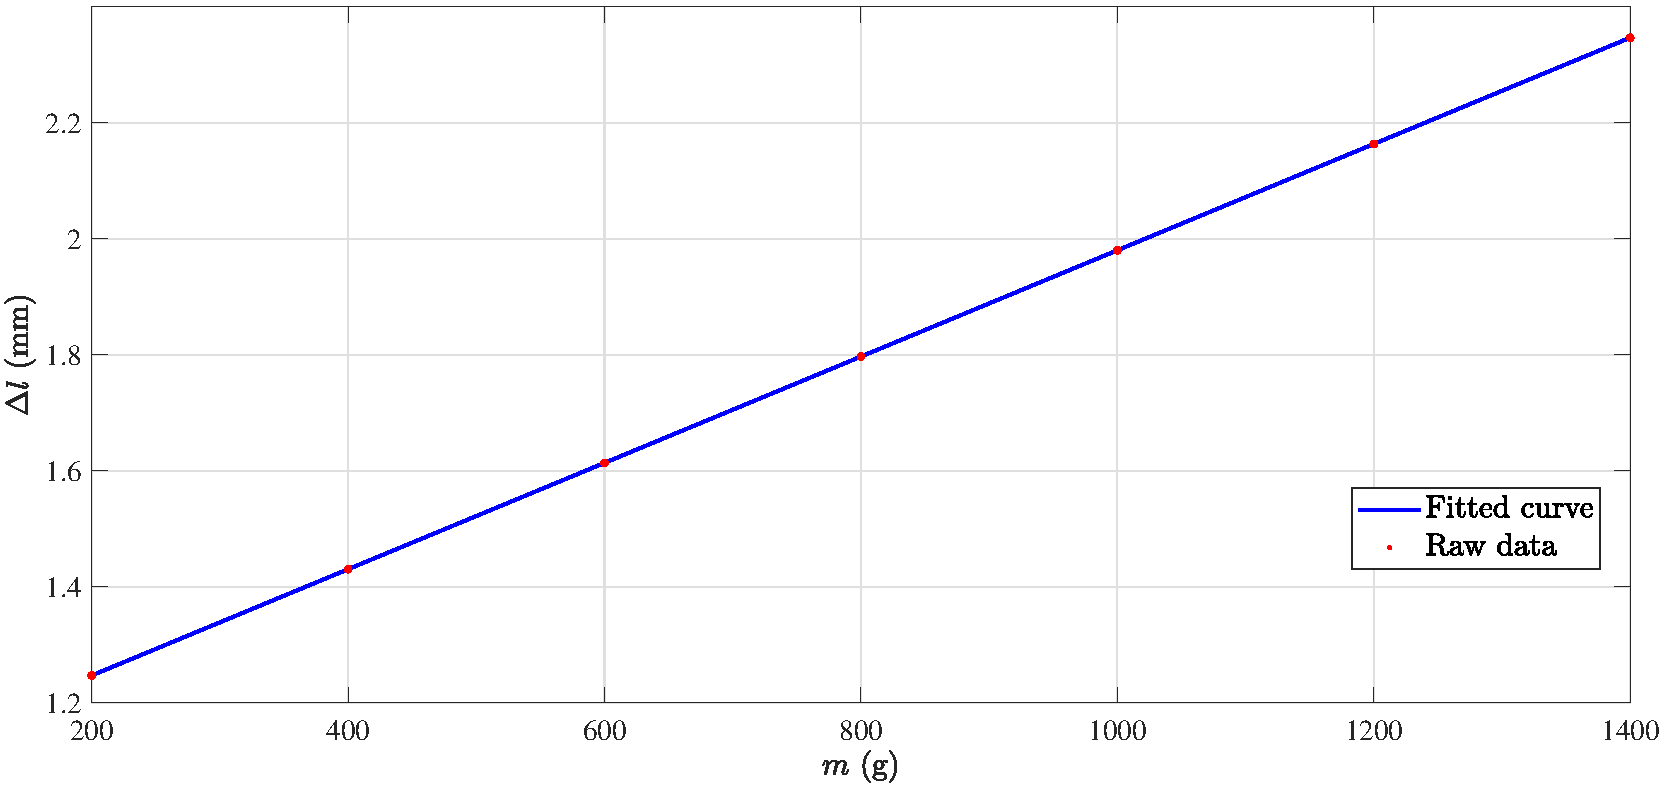
\includegraphics[width=\textwidth]{assets/2024-08-23_19-54-13.pdf}
    \caption{\textbf{作图法求杨氏模量}}\label{作图法求杨氏模量}
\end{figure}

由此计算得
	\begin{equation}
        Y=\frac{4gL}{\pi d^2k}=2.523\times10^{11}\,\mathrm{N/m^2}
    \end{equation}
与理论值的相对误差为 $9.70\ \%$.

\newpage
\section{霍尔位置传感方法测量杨氏模量}

\subsection{实验目的}
\subsection{实验器材}
\subsection{实验原理}
\subsubsection{霍尔位置传感器的定标}

霍尔元件置于磁感强度为$ B $的磁场中,再垂直于磁场的方向上加上电流$ I $,那么在与这两者垂直的方向上将产生霍尔电势差
\begin{equation}
    U_H=K\cdot I\cdot B
\end{equation}
其中$ K $为元件的霍尔灵敏度。若保持霍尔元件的电流$ I $不变,而使其在一个均匀梯度的磁场中移动时,输出的霍尔电势差变化量为

\begin{equation}
    \Delta U_H=K\cdot I\cdot\frac{\mathrm{d} B}{\mathrm{d} Z}\cdot\Delta Z
\end{equation}
上式中$ \Delta Z $为位移量。

\begin{figure}[H]
    \centering
    \includesvg[width=0.4\textwidth]{assets/梯度均匀磁场的实现.drawio.svg}
    \caption{\textbf{梯度均匀磁场的实现}}\label{梯度均匀磁场的实现}
\end{figure}

\subsubsection{弯曲法测杨氏模量}

\subsection{实验内容}
\subsubsection{注意事项}
\subsubsection{实验步骤}
\subsection{实验结果与数据处理}
\subsubsection{数据记录}

\newpage
\section{动态悬挂法测量材料的杨氏模量}
\subsection{实验目的}
\subsection{实验器材}

\newpage
\section{思考题}
\subsection{思考题 1}
\subsection{思考题 2}

\subsection{实验总结与感想}


\end{document}

% VScode 常用快捷键:

% F2:                       变量重命名
% Ctrl + Enter:             行中换行
% Alt + up/down:            上下移行
% 鼠标中键 + 移动:           快速多光标
% Shift + Alt + up/down:    上下复制
% Ctrl + left/right:        左右跳单词
% Ctrl + Backspace/Delete:  左右删单词    
% Shift + Delete:           删除此行
% Ctrl + J:                 打开 VScode 下栏(输出栏)
% Ctrl + B:                 打开 VScode 左栏(目录栏)
% Ctrl + `:                 打开 VScode 终端栏
% Ctrl + 0:                 定位文件
% Ctrl + Tab:               切换已打开的文件(切标签)
% Ctrl + Shift + P:         打开全局命令(设置)

% Latex 常用快捷键:

% Ctrl + Alt + J:           由代码定位到PDF


